\documentclass[../stats.tex]{subfiles}
\graphicspath{{\subfix{../figures/}}}
\begin{document}
\chapter{Exploring One-Variable Data}
\section{Representing Categorical and Quantitative Variables with Graphs}
Statistics is the study of data.

Data contains information about a group of individuals. This information is organized using variables.

Individuals are objects described by a set of data. Individuals may be people but may be animals or inanimate objects.

Variables are characteristics of individuals. A variable may take on different values of different variables. Variables can be split into two types: categorical or quantitative.

Categorical variables place individuals into specific groups.

Quantitative variables take on numerical values for which it makes sense to do arithmetic operations like adding and averaging. Quantitative variables fall into two categories: discret and continuous.

Careful: just because it is a number does not automatically make it quantitative.

Discrete variables are numerical values where counting makes sense; in other words, decimals would not be an appropriate way to record the data.

Continous variables are numerical values where decimals are appropriate; it usually involves some form of measuring.

One of the easiest ways to display categorical data is with a table. Here is a list of the first 10 US presidents, their political party and their state of birth.
\begin{center}
    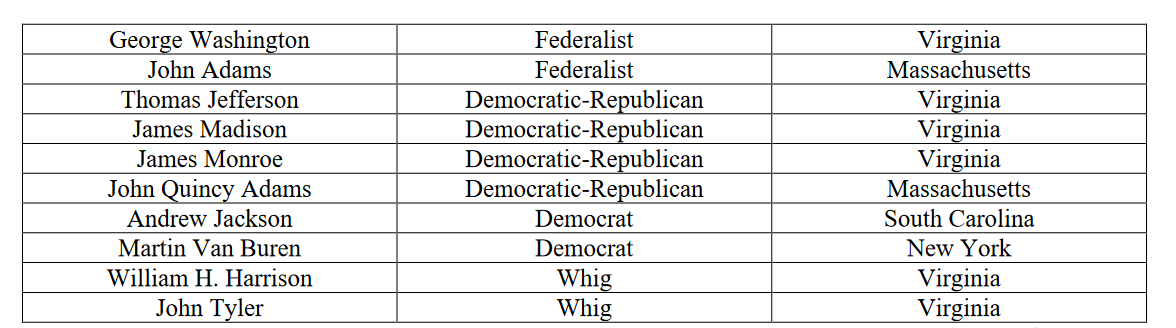
\includegraphics[width=0.8\textwidth]{1.1.1.PNG}
\end{center}

A one-way table could look like this:
\[ \begin{tabular}{c|c|c}
    \hline
    Category & Count & Relative Count\\\hline
    Federalist & 2 & 20\%\\\hline
    Democratic-Republican & 4 & 40\% \\\hline
    Democrat & 2 & 20\% \\\hline
    Whig & 2 & 20\% \\\hline
\end{tabular}\]

If you wanted to display two categorical variables at a time, you can make a two-way table. 

To better visualize the data, we can also make graphs from our data. Visualizing graphs helps get a better idea of the distribution.

The distribution of a variable tells us what value the variable takes and how often it takes these values.

Bar graphs have the following characteristics:
\begin{itemize}
    \item Label each axis clearly 
    \item The $x$-axis will contain the categorical variable and the $y$-axis will display the counts 
    \item Each category has its own bar and the bars cannot touch 
    \item Order is not important when creating the $x$-axis.
\end{itemize}

Creating a bar graph of the four political parties of the first 10 US presidents gives us the following.
\begin{center}
    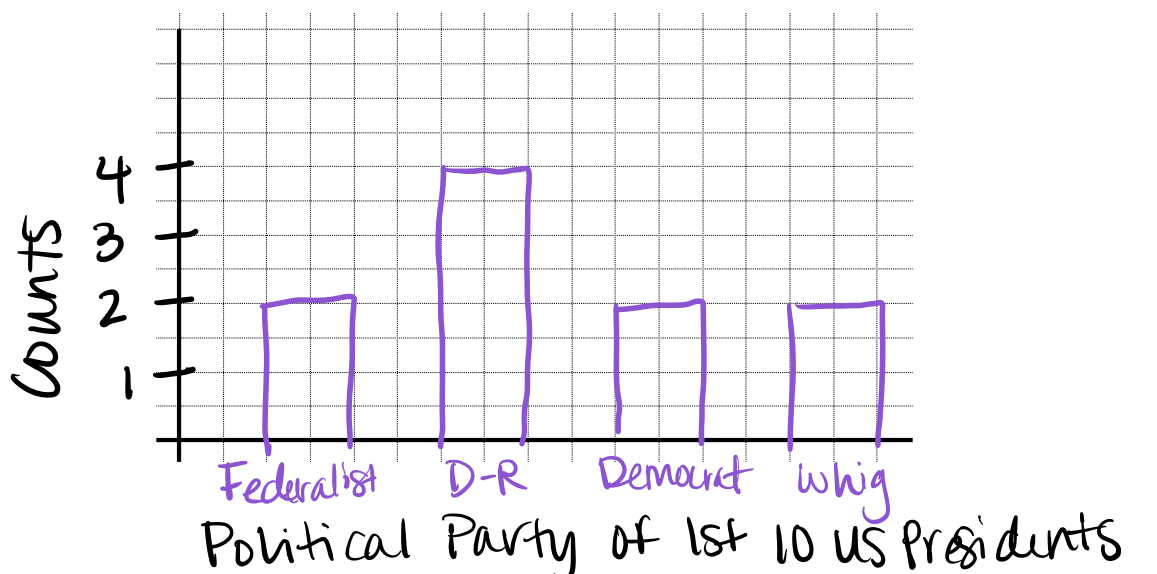
\includegraphics[width=0.8\textwidth]{1.1.2.PNG}
\end{center}

We can answer questions such as which political party was the most affiliated with, which was least affiliated with, and what the individuals and the variables of the data set are.

Talking about histograms now, let's use the table below which contains the combined scores for two weeks of NFL games.
\begin{center}
    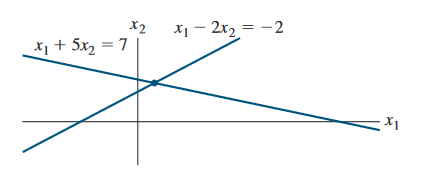
\includegraphics[width=0.8\textwidth]{1.1.3.PNG}
\end{center}

To make a histogram, we need to put the data into ``bins'' (even intervals that capture our data). We will do this first by hand by counting how many data scores are in each bin.

The lowest value is 16, the highest value is 80, so the bin width should be 14, if we want 5 bins.
\[ \begin{tabular}{c|c}
    Interval & Count\\\hline
    15-28 & 5\\\hline
    29-42 & 12\\\hline
    43-56 & 10\\\hline
    57-70 & 3\\\hline
    71-84 & 2
\end{tabular}\]
To make a histogram:
\begin{itemize}
    \item Draw rectangles for each bin with height representing the count 
    \item Bars must touch 
    \item Label the $x$-axis with the lower bound values of your bins.
\end{itemize}
\begin{center}
    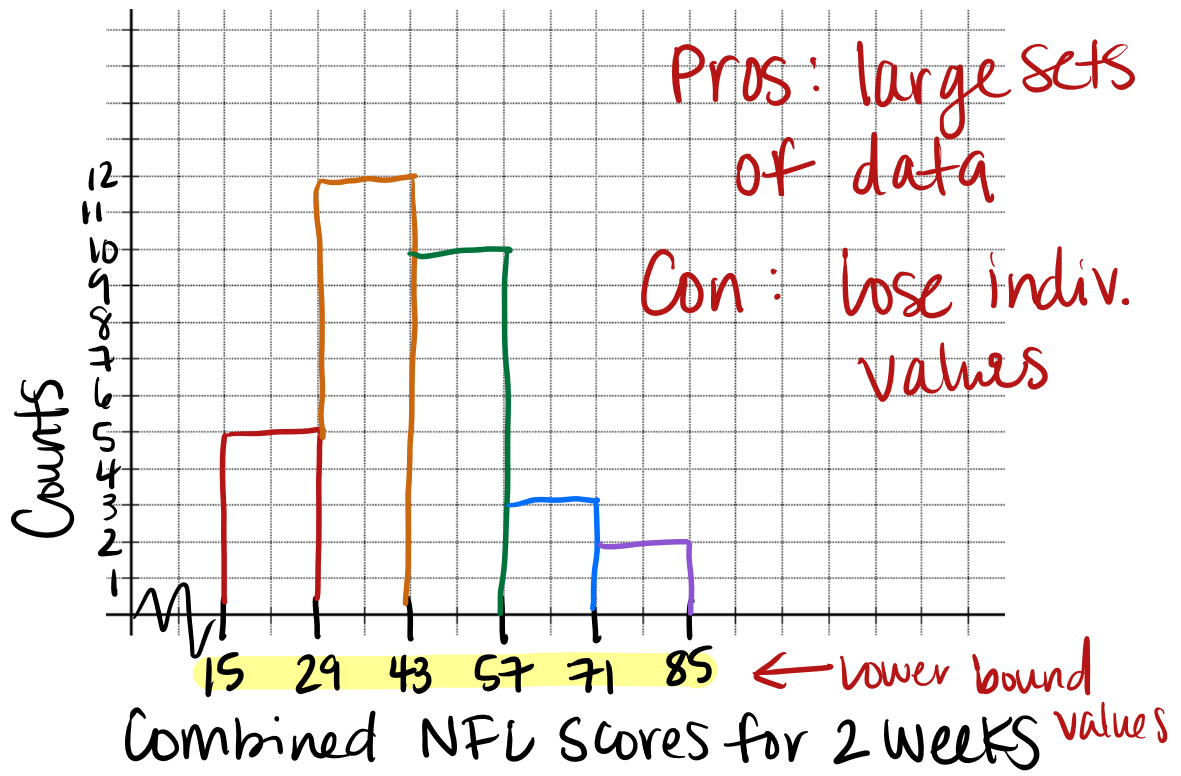
\includegraphics[width=0.8\textwidth]{1.1.4.PNG}
\end{center}

\section{Representing Quantitative Variables with Graphs}
Using the following data: we can create a stem plot. This data is the gender and average pulse rate for a set of students.
\begin{center}
    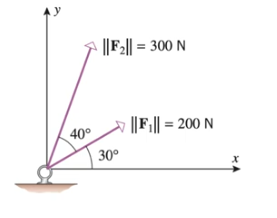
\includegraphics[width=0.8\textwidth]{1.2.1.PNG}
\end{center}
Stemplots are an alternate way of illustrating data using a semi-graph. It is similar to a histogram but, unlike a histogram, the data isn't lost. If the data has two digits, the stem is the first digit and the leaf is the second. If the data has 3 digits, the stem is the first two digits and the leaf is the third.
\begin{center}
    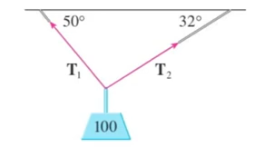
\includegraphics[width=0.8\textwidth]{1.2.2.PNG}
\end{center}

Back-to-Back stemplots are created when you can separate the data into two categories. Using the same data, we can split the data up into male and females. The stem is still the tens digit and the leaf is the ones digit.
\begin{center}
    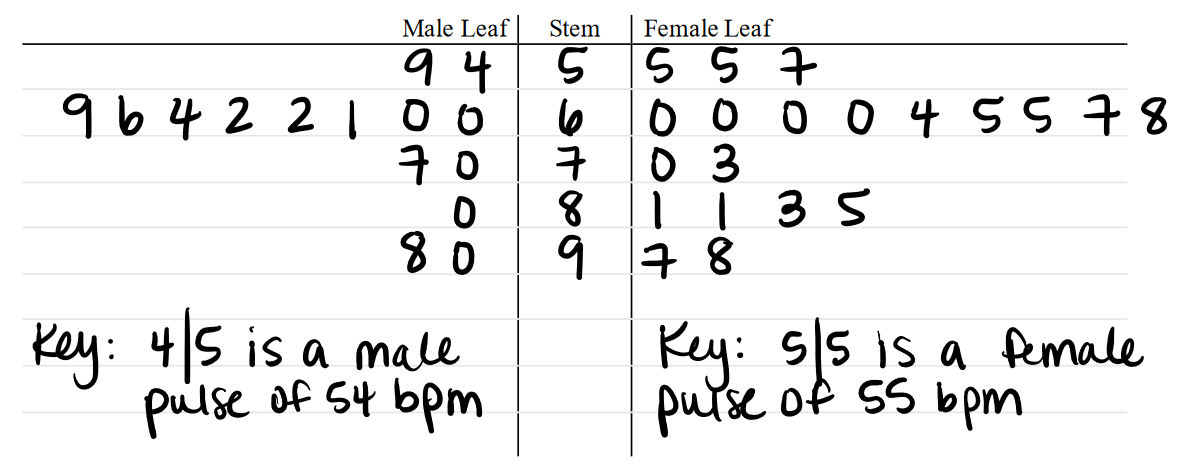
\includegraphics[width=0.8\textwidth]{1.2.3.PNG}
\end{center}

Split stemplots are the last type of stem and leaf plots. When you have too many data values on a single stem, it can be helpful to split the stem; the same way we would create more bins on a histogram if our bin width resulted in a skyscraper.

Let's say these are the test scores for an Advanced Algebra 2 Unit 1 Test:
\begin{center}
    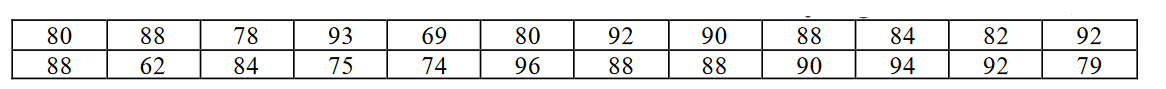
\includegraphics[width=0.8\textwidth]{1.2.4.PNG}
\end{center}
The split stem and leaf plot looks like this.
\begin{center}
    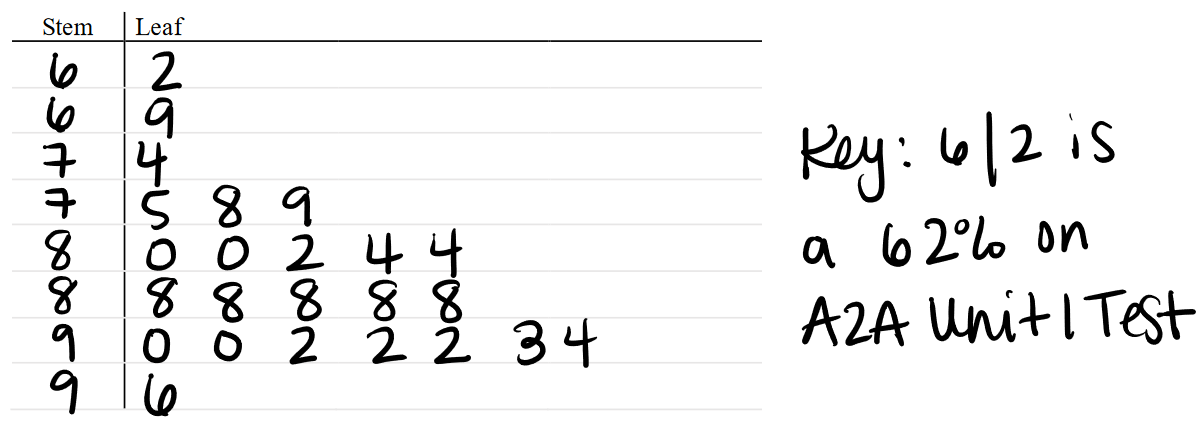
\includegraphics[width=0.8\textwidth]{1.2.5.PNG}
\end{center}

A dot plot is a very simple type of graph that involves plotting the data values, with dots, above the corresponding values on a number line. 

To construct a dot plot:
\begin{enumerate}
    \item Label your axis and title your graph. Draw a horizontal line and label it with the variable.
    \item Scale the axis based on the values of the variable.
    \item Mark a dot above the number on the horizontal axis corresponding to each data value.
\end{enumerate}

Consider the Algebra 2 Advanced quiz scores.
\begin{center}
    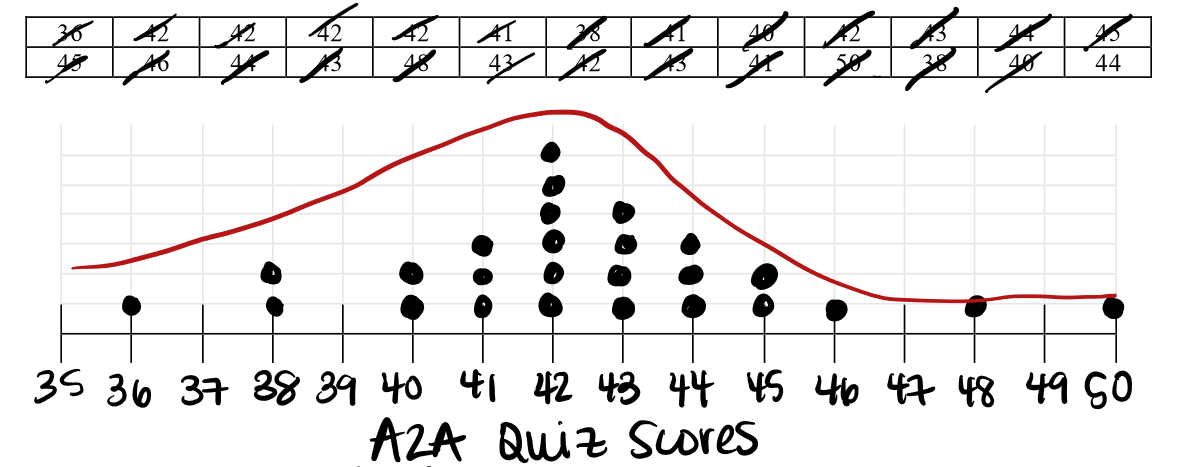
\includegraphics[width=0.8\textwidth]{1.2.6.PNG}
\end{center}

Cumulative relative frequency graphs (ogives) display percentiles.

A percentile will tell you what percent of data falls below a value.

You first must make a table of the cumulative relative frequencies in order to graph it. This can be done by finding the relative frequencies and then find the cumulative frequencies. 

The following is the ages of the 46 US presidents and their relative and cumulative frequencies.
\begin{center}
    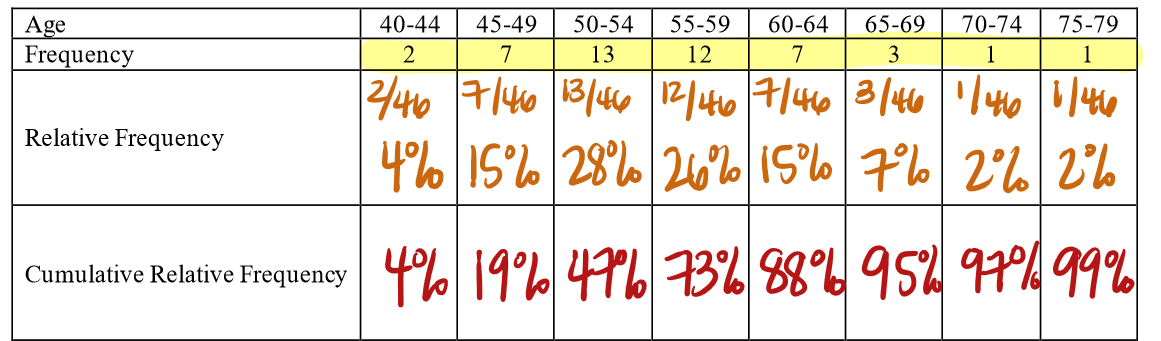
\includegraphics[width=0.8\textwidth]{1.2.7.PNG}
\end{center}

The following is what the graph looks like 
\begin{center}
    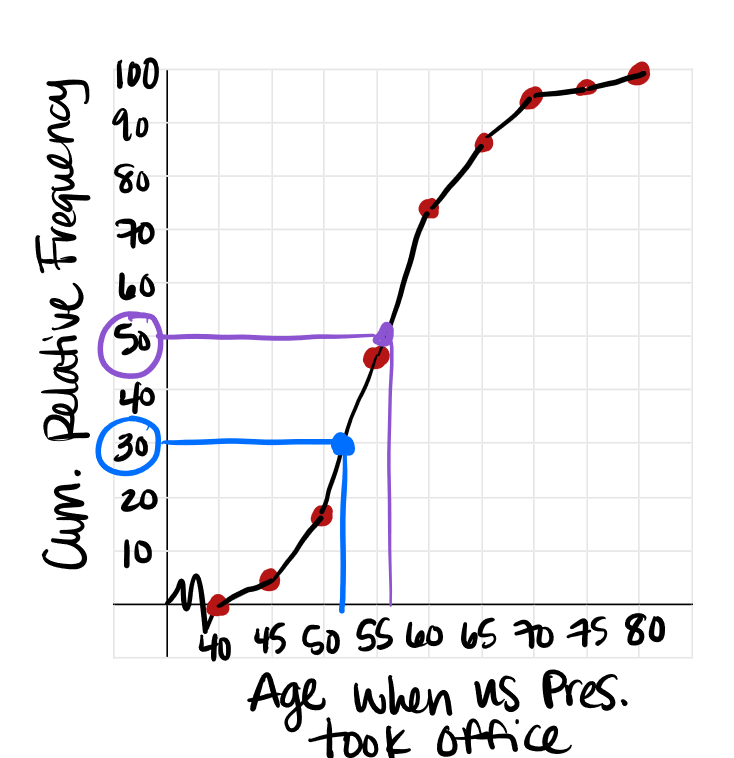
\includegraphics[width=0.8\textwidth]{1.2.8.PNG}
\end{center}
Creating an ogive:
\begin{itemize}
    \item The first interval is at 40-44, with a cumulative realtive frequency of 4\%. Since 40 is the starting interval, that starts at 0 and 4\% is graphed at 45.
    \item The next interval is 45-49, with a cumulative relative frequency of 20\%. At 45, 4\% is graph, so at 50, the 20\% will be graphed.
    \item This pattern continues until 100\% is graphed at 80.
\end{itemize}

Answer the following questions with the ogive:
\begin{enumerate}
    \item At approximately what age is the 30th percentile? What does this mean in the context of the problem?
    \item Richard Nixon was the 37th president and was 56 years old when he was inaugurated. Approximately what percentile is this and what does it mean in the context of the problem? 
\end{enumerate}

\section{Describing Distributions of Quantitative Variables}
In AP Statistics, to describe a distribution of a quantitative variable, we use the acronym SOCS:
\begin{itemize}
    \item S: Shape 
    \item O: Outliers 
    \item C: Center 
    \item S: Spread
\end{itemize}

After we graph, describing what we see helps identify patterns and answers questions about the data.

Once the distribution is graphed, the first thing we identify is the shape.
\begin{center}
    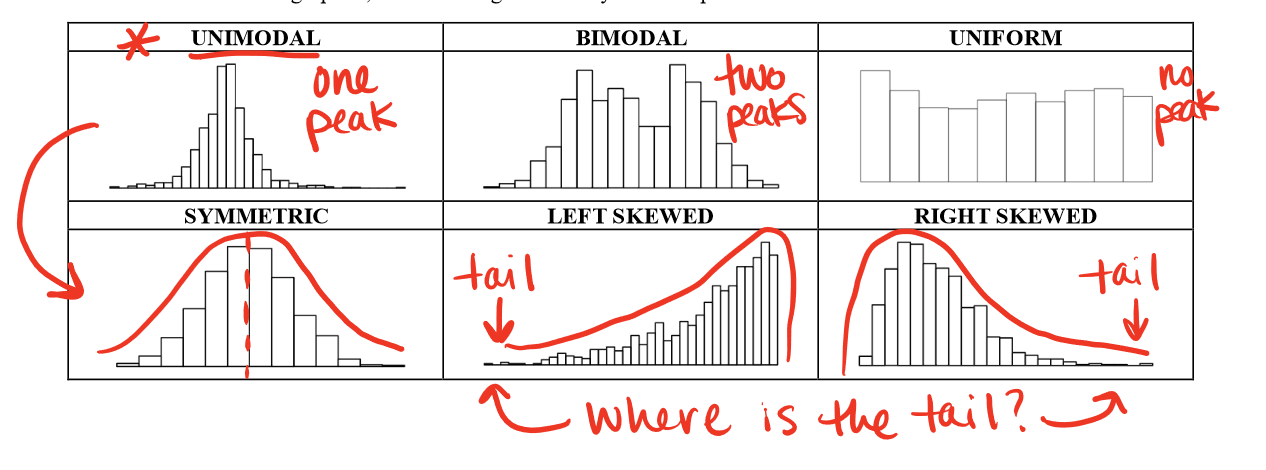
\includegraphics[width=0.8\textwidth]{1.3.1.PNG}
\end{center}

There are three measures of center in statistics: mean, median, and mode.

The following data is the number of siblings for a group of students.
\begin{center}
    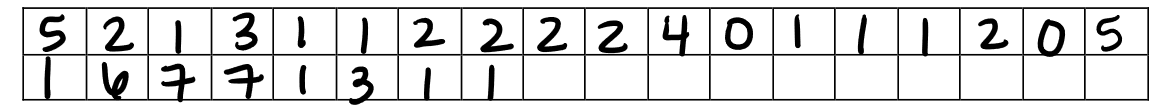
\includegraphics[width=0.8\textwidth]{1.3.2.PNG}
\end{center}

Mean is symmetric. The formula for mean is 
\[ \overline{x}=\frac{\sum x_i}{n} \]
Where $\overline{x}$ is the mean of the sample, $x_i$ is each individual observation, $n$ is the number of observations, and $\sum$ is notation for a summation.

The mean of this data would be 2.38 siblings.

The reason we do not always use the mean to describe the center is the inclusion of outliers in the data set.

For example, if we had 7 scores of 90, 92, 94, 98, 86, 88, and 0, the mean would be 78.29\%. Removing the outlier, the mean increases to 91.33\%. The outlier is bringing the mean down in this instance.

The mean is called non-resistant. This means that the mean is strongly influenced by extreme values.

Median - skewed. Luckily, we have another measure of center that is resistant, meaning that if there are extreme values in a data set, the measure of center will not be affected by it.

The median is found by ordering the data and then finding the middle value in that list.

Looking at the set of 7 scores above, the median would be 90\%. This shows that the median is greater than the mean.

Whenever there are extreme values or outliers, the median is the better measure of center compared to the mean.

The last measure of center is perhaps the most useless: the mode. It find the most occurring value in a data set. The idea of having this as a measure of centere comes from having a symmetric, unimodal distribution, where the most occurring value happens in the middle. However, as we have seen, there are many shapes to different distributions and the most occurring doesn't always occur in the middle.

Summary:
\begin{center}
    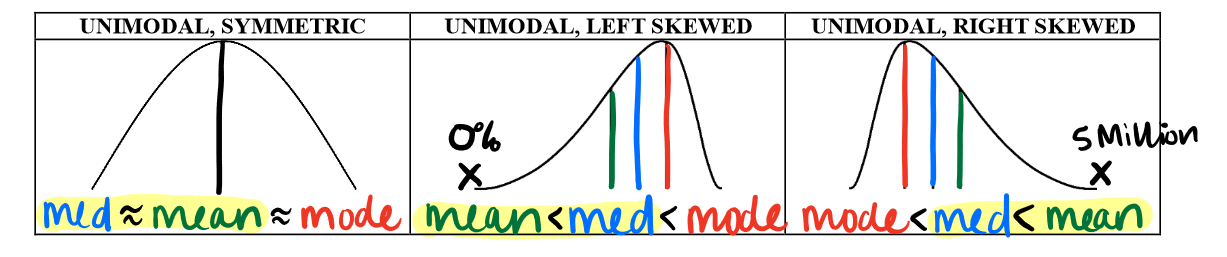
\includegraphics[width=0.8\textwidth]{1.3.3.PNG}
\end{center}

Spread (variability): There are three common measures of spread in statistics: range, standard deviation, and IQR.

The range is the difference between the maximum value and minimum value.

The standard deviation is the average deviation of an observation from the mean of the data set.
\[ s_x = \sqrt{\frac{\sum (x_i-\overline{x})^2}{n-1}} \]
where $s_x$ is the standard deviation of the sample, $\overline{x}$ is the mean of the sample, $x_i$ is each individual observation, $s_x^2$ is the variance of the sample, $n$ is the number of observations, and $\sum$ is the summation notation.

Within the standard deviation, we calculate something called the variance which is the average squared deviation. We can find the variance from the standard deviation by squaring both sides to eliminate the square root.

In context the standard deviation is ``The {quantitative variable} typically varies from the mean by {standard deviation} {units}.''

Standard deviation should only be used as your measure of spread when the mean is your chosen measure of center.

The standard deviation has the following additional properties:
\begin{itemize}
    \item The standard deviation is always positive.
    \item The standard deviation is 0 when all observations are equal.
    \item The standard deviation has the same units of measure as the original variable measured.
    \item The standard deviation is non-resistant, meaning that a few outliers will make it large.
    \item The greater the standard deviation, the greater the distribution.
\end{itemize}

The last measure of spread is Inter-Quartile Range (IQR) and uses percentiles to describe the spread of the distribution.

Here are some other percentiles:
\begin{itemize}
    \item 0th percentile: minimum - lowest value in a data set 
    \item 25th percentile: Quartile 1 or Q1 - 25\% of the data set is below this value 
    \item 50th percentile: Median - middle value in a data set 
    \item 75th percentile: Quartile 3 or Q3 - 75\% of the data set is below this value 
    \item 100th percentile: maximum - highest value in a data set 
\end{itemize}

These 5 numbers make up what is called the Five Number Summary. To calculate these values by hand, place the observation in ascending order and find the median. Then find the middle value to the left and right of your median to identify your quartiles.

\begin{example}
    Here is the data from a previous class about how many hours of sleep they got before the first day of school.
    \begin{center}
        2 4.5 5 5 6 6 6.5 7 7 7 7 7 7 7 7.5 8 8 8 8 8 8.5
    \end{center}

    From this, the minimum is 2, the Q1 value is 6, the median is 7, the Q3 value is 8, and the max value is 8.5.

    The IQR is 2 hours.
\end{example}

An outlier is an individual piece of data that falls outside the overall pattern of the distribution.

When an outlier occurs, we must find out why it occurs. Many times, it occurs because of a mistake. Outliers can be eliminated from the data if there is a good reason. However, if you are unsure then you cannot just remove the data point.

Most of the time, the AP exam wants you to comment on visual outliers from a graph of quantitative variable.

Using the five-number summary and the IQR, we also have a numerical way of determining if a point is an outlier.
\begin{enumerate}
    \item Find the five-number summary.
    \item Find the IQR.
    \item Compute Q1 - (1.5*IQR). Any data below that number is an outlier.
    \item Compute Q3 + (1.5*IQR). Any data above that number is an outlier.
\end{enumerate}

\begin{example}
    Literary scholars sometimes use the distribution of word lengths in a work as a test of authenticity. Here are the words lengths for the first 26 words on a randomly-selected page from Toni Morrison's Song of Solomon.
    \begin{center}
        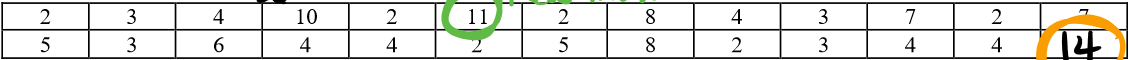
\includegraphics[width=0.8\textwidth]{1.3.4.PNG}
    \end{center}

    (a) Mathematically check for outliers in your data.

    The IQR is 4, so any numbers outside the bound of -3 to 13 are outliers. There is an outlier at 14 words.

    The five number summary can also be used to create a boxplot or a modified boxplot (one that shows outliers).

    (b) Create a boxplot and a modified boxplot for your data.
    \begin{center}
        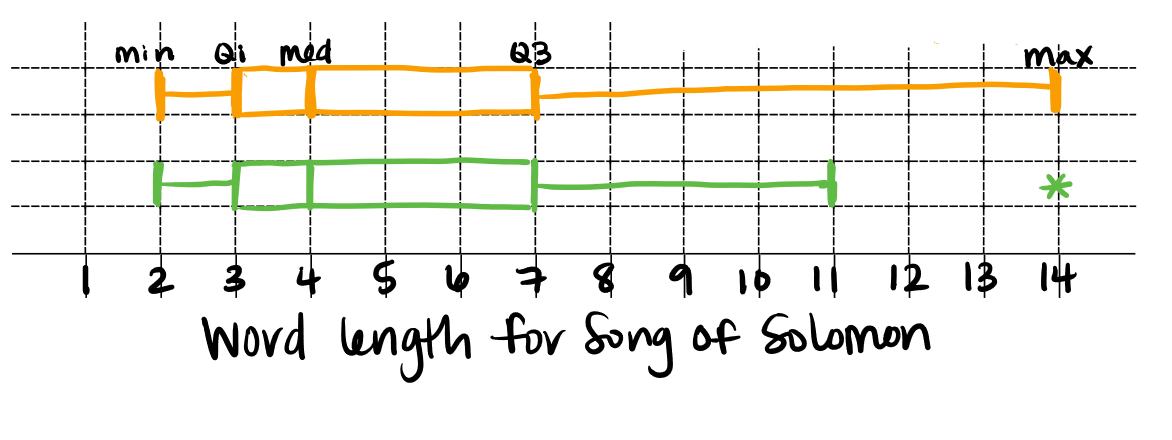
\includegraphics[width=0.8\textwidth]{1.3.5.PNG}
    \end{center}
\end{example}


\section{Comparing Distributions of Quantitative Variables}
In the world of statistics, it is not enough to just report the graph or just report the summary statistics. The graph alone might not give us all the information we need to make a valid conclusion.
\begin{example}
    Do teachers in New York get paid too much? The graph below shows the average teacher salary for each state.
    \begin{center}
        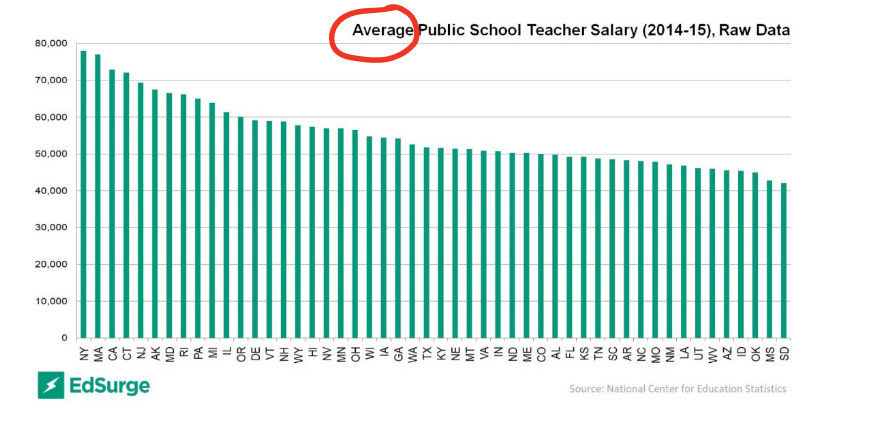
\includegraphics[width=0.8\textwidth]{1.4.1.PNG}
    \end{center}
    The graph shows that teachers in New York State make almost double than teachers in South Dakota. Is this a valid conclusion or is the graph not telling the whole story?

    The cost of living is higher in New York and we are looking at the ``average'' which is non-resistant.

    The summary statistics might not give us all the information we need to make a valid conclusion.
\end{example}

\begin{example}
    The mean teacher salary in the state of California is \$84,531. This lets us know that teachers are making above the median income for everyone in California, which is \$78,672. Is this a valid conclusion or are the summary statistics
    not telling the whole story?

    The mean is non resistant which means some places have more well paying districts or more experienced teachers.

    This is skewed right.
\end{example}

Being a statistics student means you must report both a visual display of the data as well as detailed summary statistics when asked to ``describe the distribution''.

First: Create your Graph (If it is not given)
\begin{itemize}
    \item Is your data categorical? Use a bar graph! 
    \begin{itemize}
        \item Two variables will require a segmented bar graph or mosaic plot.
    \end{itemize}
    \item Is your data quantitative?
    \begin{itemize}
        \item Discrete? Use a dot plot, stem plot, or boxplot.
        \item Continuous? Use a histogram or boxplot.
        \item Two variables will require a scatterplot.
    \end{itemize}
\end{itemize}
Cumulative frequency graphs will usually take too long to create on the AP exam, but remember if you are interested in percentile positions, then you can create these graphs as well!

Second: Summarize your findings. 
\begin{itemize}
    \item Shape - Skewed, Symmetric, Bimodal, etc. 
    \begin{itemize}
        \item Be as specific as possible and combine shape terms if you can.
    \end{itemize}
    \item Outliers - an individual observation that falls outside the overall pattern of the graph.
    \begin{itemize}
        \item You will just have to comment on if there are any visual outliers. You do not have to do the outlier test unless instructed.
    \end{itemize}
    \item Center - Mean and Median 
    \begin{itemize}
        \item Use the mean, unless the distribution is skewed or has outliers. 
        \item Unless asked for otherwise, a verbal description of the center is fine.
    \end{itemize}
    \item Spread - Range, Standard Deviation, IQR 
    \begin{itemize}
        \item If you describe the center with the mean, comment on the standard deviation.
        \item If you describe the center with the median, comment on the range or IQR.
    \end{itemize}
\end{itemize}
When the problems asks to ``compare the distributions'', follow the steps above, but make sure you are using comparison words to compare the distributions.

\pagebreak
\begin{example}
    The following data are for two popular songs on the Billboard Top 100. The length of each word in the song was recorded and below shows the number of words with the corresponding number of letters.
    \begin{center}
        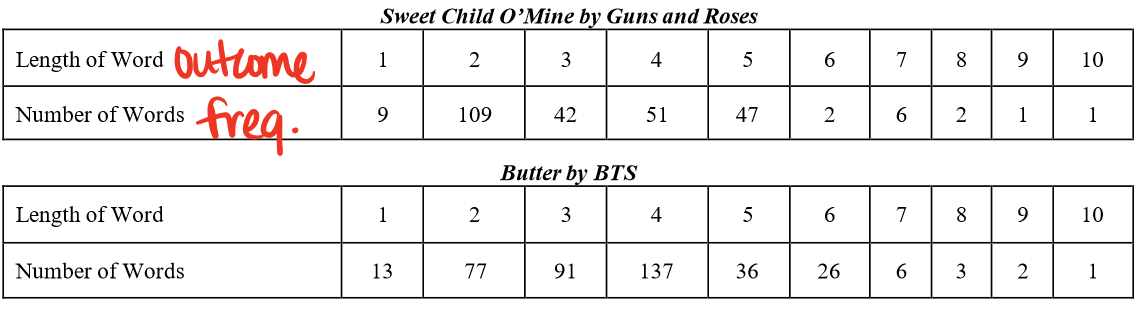
\includegraphics[width=0.8\textwidth]{1.4.2.PNG}
    \end{center}
    (a) Determine the five number summary for each data set.

    Sweet Child: min = 1, Q1 = 2, med = 3, Q3 = 4, max = 10 

    Butter: min = 1, Q1 = 3, med = 4, Q3 = 4, max = 10

    (b) Below are the graphs of the two distributions. Write a few sentences comparing the distributions.
    \begin{center}
        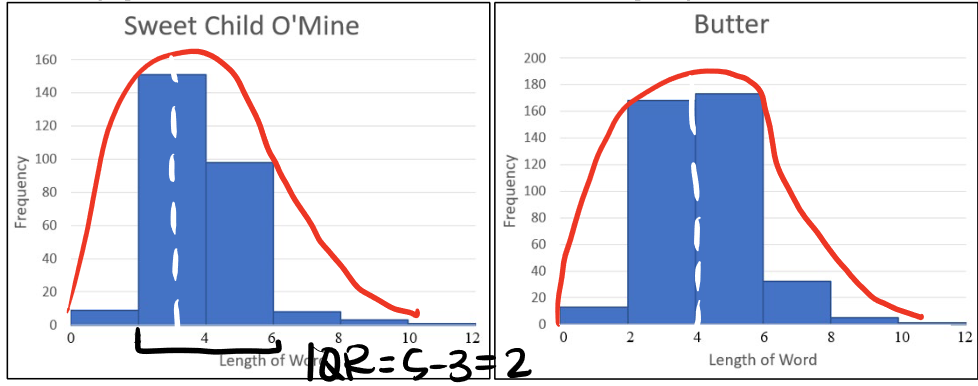
\includegraphics[width=0.8\textwidth]{1.4.3.PNG}
    \end{center}
    \begin{itemize}
        \item Both distributions of word lengths are right skewed.
        \item Neither distribution has visible outliers.
        \item The median of Sweet Child is 3 letters which is smaller than the median of Butter which is 4 letters.
        \item The IQR of Sweet Child is 2 letters which is larger than the IQR of Butter which is 1 letter.
    \end{itemize}

    (c) There are two ``rules'' we used to mathematically determine outliers. Method A is the 1.5 x IQR rule and Method B is the two standard deviation rule.
    
    (i) Using method A, determine the outliers that are present in the Sweet Child O'Mine distribution. Justify your answer.

    The lower bound is -1, upper bound is 7. There are four outliers of 8, 8, 9, and 10 letters.

    (ii) The mean numenr of letters in the Butter distribution is 3.62 and the standard deviation is 1.42. Using method B, determine the outliers that are present in the Butter distribution. Justify your answer.

    The lower bound would be 0.78 and the upper bound would be 6.46 in this. There are 12 outliers, 6 with 7 letters, 3 with 8 letters, 2 with 9 letters, and 1 with 10 letters.

    (d) Explain why method A is better for determining outliers than method B in these distributions.

    Method A is better because both distributions are right skewed. Method B uses statistics that are strongly affected by outliers.
\end{example}


\section{Z-Scores and the Empirical Rule}
The normal distribution is bell-shaped, and we draw a density on curve on the graph below. You acn see that this curve will approximate the data, not describe it perfectly.
\begin{center}
    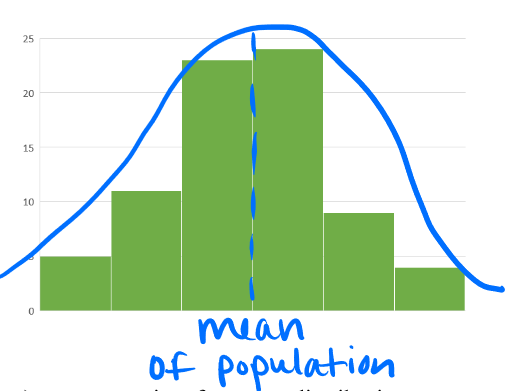
\includegraphics[width=0.8\textwidth]{1.5.1.PNG}
\end{center}
Density curves, like distributions, come in many shapes. A density curve is often a good description of the overall pattern of a distribution.

Normal distributions are appropriate for many distributions whose shapes are unimodal and approximately symmetric.

The mean is written as $\mu$, the standard deviation is $\sigma$ and and the normal distribution is described as $N(\mu,\sigma)$

A normal distribution density curve has the following properties:
\begin{itemize}
    \item Symmetric around the mean 
    \item Mean = med = mode 
    \item 50\% of observations are less than the mean 
    \item 50\% of observations are greater than the mean 
    \item The standard deviation tells us how measurements for a group of observations are spread out from the mean 
    \item In a normal distribution, approximately all of the data lies within 3 standard deviations above and below the mean 
\end{itemize}

\pagebreak
\begin{example}
    The heights of American women aged 18 to 24 years old with a mean of 65.6 inches and a standard deviation of 2.5 inches. Assuming the population is normally distributed, draw a normal curve and label 3 standard deviations out on either side.
    \begin{center}
        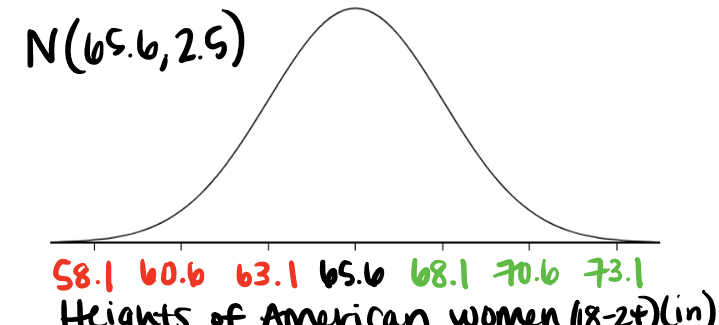
\includegraphics[width=0.8\textwidth]{1.5.2.PNG}
    \end{center}
\end{example}

In a normal distribution, we can describe the variability of the data in terms of probabilities.
\begin{itemize}
    \item 68\% of data is likely to be within 1 standard deviation around the mean 
    \item 95\% of data is likely to be within 2 standard deviations around the mean 
    \item 99.7\% of data is likely to be within 3 standard deviations around the mean 
\end{itemize}
\begin{center}
    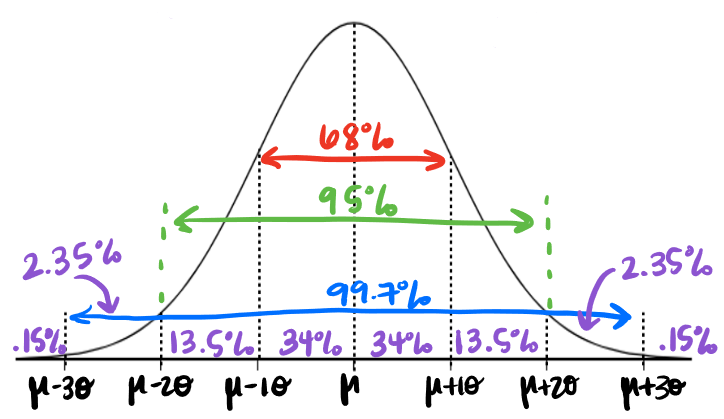
\includegraphics[width=0.8\textwidth]{1.5.3.PNG}
\end{center}
These three percentages 68-95-99.7 describe the empirical rule. These approximations can be used with the symmetry of a normal distribution to approximate proportions of data.

\pagebreak
\begin{example}
    For the following draw a normal distribution and use the empirical rule to answer the question.

    (a) The mean test score on the Unit 1 Test was an 82 with a standard deviation of 4. 95\% of the test scores were between what two scores?

    74 and 90.
    \begin{center}
        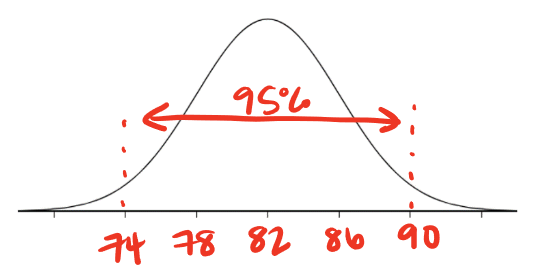
\includegraphics[width=0.6\textwidth]{1.5.4.PNG}
    \end{center}

    (b) The mean age at the concert was 38 years old with a standard deviation of 5.5 years. What percent of the concert goers were between 32.5 years old and 43.6 years old?

    68\%
    \begin{center}
        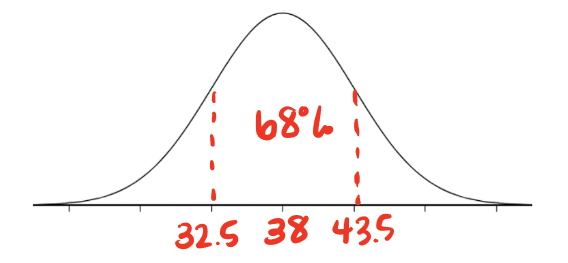
\includegraphics[width=0.6\textwidth]{1.5.5.PNG}
    \end{center}

    (c) The mean test score on the Unit 1 Test was a 82 with a standard deviation of 4.
    (i) What percent of test scores fell below a 74?

    2.5\%

    (ii) What percent of test scores fell above a 78?

    84\%
    \begin{center}
        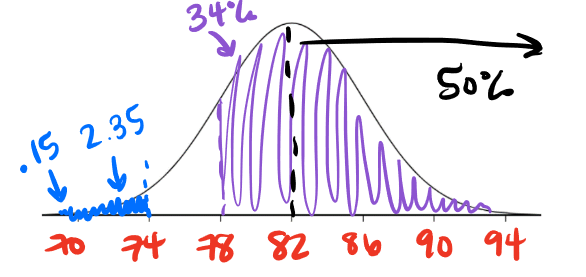
\includegraphics[width=0.6\textwidth]{1.5.6.PNG}
    \end{center}
\end{example}

The location of an observation in relationship with its mean is one that is asked often. So often, in fact, we have a method of calculating how far away an observation is from its mean.
This method is called standardizing, and it is the process of counting how many standard deviations above or below the mean an observation falls.

Let's say you scored a 86\% on a test, and 83\% was the class mean with a standard deviation of 4.5\%.

Subtracting your score from the mean gives the distance from the mean, and to determine if this distance is ``typical'', divide by the standard deviation to see how many standard deviations it is away from the mean. The number you get is the number of standard deviations from the mean an observation is, or a z-score.

The z-score would be 0.67 in this case, or your score would be 0.67 standard deviations above the mean.

If $x$ is an observation from a distribution that has known mean and standard deviation, the z-score for $x$ is:
\[ z=\frac{\text{value-mean}}{\text{SD}}=\frac{x-\mu}{\sigma} \]
\begin{itemize}
    \item A z-score tells us how many standard deviations from the mean an observation falls and in what direction.
    \item Observations larger than the mean have positive z-scores.
    \item Observations smaller than the mean have negative z-scores.
\end{itemize}

\begin{example}
    Female shoe sizes are approximately normally distributed with a mean of 8 and a standard deviation of 0.75. Find and interpret the z-score of a female with a size 6 shoe.

    The z score can be calculated as -2.67. A female with a size 6 shoe is 2.67 standard deviations below the mean women shoe size.
\end{example}

\begin{example}
    Joe is 74'' tall. The average height of an adult male is 70'' with a standard deviation of 2.5''. Find and interpret the z-score for Joe's height.

    The z score is 1.6. Joe is 1.6 standard deviations above the mean height of adult males.
\end{example}

\begin{example}
    Corbin scored 1100 on the SAT in 2020. The distribution of SAT scores in 2020 was normally distributed, 
    with a mean score of 1083 and a standard deviation of 194. Corbin also took the ACT in 2020 and earned a score of 23. The 2020 ACT scores were normally distributed with 
    a mean of 21 and a standard deviation of 1.62. On what standardized test did Corbin scored better on?

    The z-score for the SAT is 0.09 and for the ACT it is 1.23. Corbin scored better on the ACT because he was more standard deviations above the mean.
\end{example}


\section{The Standard Normal Curve}
How do we determine percentages if they do not follow the Empirical Rule? We standardized the normal curve.

The curve we created is called the standard normal curve and any data set that is normally distributed can be standardized into the standard normal curve.

If you have a standard curve, we have a standard set of measurements we can use to determine what percentage of data falls above, below, or between specific z-scores.

We can determine what percentage of data falls above, below, or between specific z-scores using our TI-84 calculator.
\begin{center}
    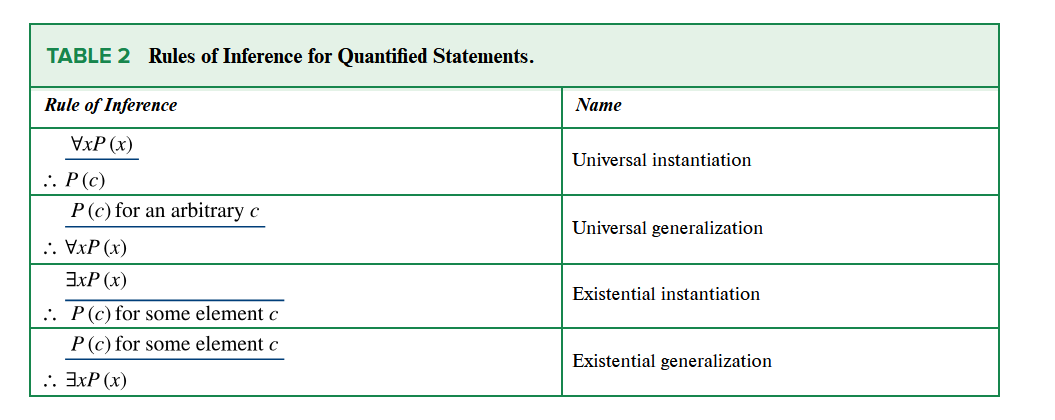
\includegraphics[width=0.8\textwidth]{1.6.1.PNG}
\end{center}

\begin{example}
    (a) What percent of data is below a z-score of 0.54?

    70.54\%

    (b) What percent of data is above a z-score of 0.17?

    43.25\%

    (c) What percent of data lies between z = -1.64 and z = 2.33?

    93.96\%

    (d) What percent of data lies outside z = -1.64 and z = 2.33?

    6.04\%
\end{example}

\begin{example}
    On a typical Saturday, Kroger reports that the mean amount of money spent by customers is \$27.21 and a standard deviation of \$7.93. The distribution is approximately normal.

    (a) What percentage of people spend less than \$20?

    The z score is -0.91, so this is the upper bound. Normalcdf gives us 18.14\%.

    (b) What percentage of people spend above \$40?

    The z-score is 1.61, so the percentage is 5.37\%.

    (c) How many people spend between \$25 and \$30?

    Note: On a MCQ question, you do not need to translate these values to z-scores. If you use the original values for the mean and standard deviation and use the numbers on this question as the bounds, you get an equivalent answer. The percentage is 24.73\%.
\end{example}

\pagebreak
\begin{example}
    On a typical school night, students get an average of 8 hours of sleep with a standard deviation of 1.2 hours. How many hours of sleep would a student need to get to be in the 75th percentile?

    Step 1: Find the z-score.

    The 75th percentile means at or below 75\%, the z-score would be expected to be positive.
    \begin{center}
        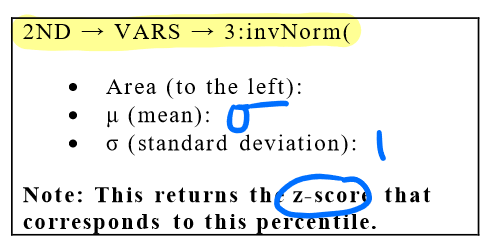
\includegraphics[width=0.8\textwidth]{1.6.2.PNG}
    \end{center}
    The z-score is 0.67.

    Step 2: Find the raw data.

    Take your z-score and the mean and standard deviation of your distribution, and use the z-score formula to solve for $x$, the raw data value.

    Solving for $x$ in $0.67=\frac{x-7}{1.2}$ gives $x=7.804$ hours of sleep.
\end{example}

\begin{example}
    If $z=-2.3$, $\mu=23$, and $\sigma = 5$, what is your $x$-value?

    Do the same process as above, and you get $x=11.5$.
\end{example}

\begin{example}
    (a) If you have 35\% of the data lying symmetrically in the middle of your distribution, what are your z-scores?

    If you have 35\% of the data in the middle, the z-scores will be the same value, but opposite signs due to symmetry. The percentages of each tail is $1-0.35=0.325$.

    Using invNorm to get the z-score gives $z=-0.45$ and $z=0.45$.
\end{example}

\pagebreak
\begin{example}
    (a) On the most recent test, a student scored in the 40th percentile. The mean of the test scores was an 85 and the standard deviation was 1.5. What was the student's score?

    Using invNorm gives $z=-0.25$, and finding for $x$ gives $x=84.625$.

    (b) An automobile dealer finds that the average price of a previously owned vehicle is \$8,256. He decides to sell cars that will appeal to the 
    middle 60\% of the market in terms of price. Find the maximum and minimum prices of the cars the dealer will sell.
    The standard deviation is \$1,150 and the variable is normally distributed.
    
    The tails would be $1-0.60=0.40/2 = 0.20$. Using invNorm for this gives z scores of $-0.84$ and $z=0.84$, so the $x$ values found would be $7290$ and $9222$.

    The minimum price is \$7290 and the maximum price is \$9222.
\end{example}




\end{document}